%   % !TEX root = ../../VIII,3_Rahmen-TeX_9-0.tex
%  
%   Signatur/Tex-Datei:	LH_37_05_144-145
%   RK-Nr. 	57267_2
%   Überschrift: 	(keine)
%   edlabels:			29	+1 (Referenz)		
%   Diagramme: 		5
%
%   NB: 				Auf 145v+144r Stück 57268 (Specimina artis...), auf 144r 57267_1
%
%
%
\selectlanguage{ngerman}
\frenchspacing
%
\begin{ledgroupsized}[r]{120mm}
\footnotesize
\pstart
\noindent\textbf{Überlieferung:}
\pend
\end{ledgroupsized}
%
\begin{ledgroupsized}[r]{114mm}
\footnotesize
\pstart \parindent -6mm
\makebox[6mm][l]{\textit{L}}%
Auszüge mit Bemerkungen aus
\protect\index{Namensregister}{\textso{Huygens} (Hugenius, Ugenius, Hugens, Huguens), Christiaan 1629\textendash1695}\textsc{C.~Huygens}, 
\cite{00529}\glqq Regles du mouvement dans la rencontre des corps\grqq,
\cite{00157}\textit{JS}, 18.~März 1669, S.~22\textendash24:
LH~XXXVII~5~Bl.~144\textendash145. %ggf. (unsere Druckvorlage).
Ein Bogen~2\textsuperscript{o};
Wasserzeichen in der Mitte von Bl.~145;
Papiererhaltungsmaßnahmen;
Papierbruch an den Blatträndern mit Textverlust.
Eineindrittel Seiten auf Bl.~144~v\textsuperscript{o} und 145~r\textsuperscript{o} sowie einige Zeilen im Randbereich von Bl.~144~r\textsuperscript{o}.
Textfolge: Bl.~144~v\textsuperscript{o}; Rechnungen auf 144~r\textsuperscript{o}; 145~r\textsuperscript{o}.
Bl.~144~r\textsuperscript{o} überliefert N.~\ref{57267_1},
Die unteren zwei Drittel von Bl.~145~r\textsuperscript{o} und der obere Rand von Bl.~145~v\textsuperscript{o} überliefern N.~\ref{57267_3},
Bl.~145~v\textsuperscript{o} und der untere linke Bereich von Bl.~144~r\textsuperscript{o} überliefern N.~\ref{57268}.
\pend
\end{ledgroupsized}
%
\begin{ledgroupsized}[r]{114mm}
\footnotesize
\pstart
\parindent -6mm
\makebox[6mm][l]{\textit{E}}%
(tlw.) \textsc{Fichant} 1994, S.~357\textendash361\cite{01056}.
\pend%
\end{ledgroupsized}
%
%
\selectlanguage{french}
\frenchspacing
% \newpage%
\vspace{8mm}
%
\count\Bfootins=1100%
\count\Afootins=1100%
\count\Cfootins=1100
\pstart%
\normalsize%
\noindent%
\edlabel{37_05_144-145_24a}%Anfang der Besprechung von Huygens
\lbrack144~v\textsuperscript{o}\rbrack\
\pend
%
% Überschrift
\pstart
\centering
\edtext{Regle de Mons.\ Hugens\protect\index{Namensregister}{\textso{Huygens} (Hugenius, Ugenius, Hugens, Huguens), Christiaan 1629\textendash1695}}%
{\lemma{}\Bfootnote{Regle de Mons.\ Hugens \textit{erg.\ L}%
}\lemma{Regle de Mons.\ Hugens}\Cfootnote{\protect\index{Namensregister}{\textso{Huygens} (Hugenius, Ugenius, Hugens, Huguens), Christiaan 1629\textendash1695}\textsc{C.~Huygens}, \cite{00529}\glqq Regles du mouvement dans la rencontre des corps\grqq, \cite{00157}\textit{JS} (Pariser Ausgabe), 18.~März 1669, S.~22\textendash24 (\cite{00113}\textit{HO} XVI, S.~179\textendash181).%
}}.
\pend
\vspace{\baselineskip}
%
%
\pstart\noindent
\hspace{1mm}\hspace{-1mm}% Trick, weil \edlabel nicht zu \par-Beginn sein darf
\edlabel{37_05_144-145_1a}\edtext{}{% C-Footnote – Huygens-Stelle
{\xxref%
{37_05_144-145_1a}{37_05_144-145_1b}}%
\lemma{\textit{La regle} \lbrack...\rbrack\ \textit{l'autre}}%
\Cfootnote{%
\cite{00529}a.a.O., §4, S.~22.%
}}%
\textit{La regle generale pour determiner le mouvement qu'acquierent les corps durs%
\protect\index{Sachverzeichnis}{corps dur} par leur rencontre directe,%
\protect\index{Sachverzeichnis}{rencontre directe}\protect\index{Sachverzeichnis}{rencontre} est telle:}
\pend \pstart
\textit{Soyent les corps A et B desquels  A soit meu avec la vistesse AD, et que B aille à sa rencontre%
\protect\index{Sachverzeichnis}{rencontre} ou bien vers le même costé avec la vistesse BD ou que mêmes il soit en repos}\lbrack,\rbrack\ 
%
\textit{le point D en ce cas estant le même que B. Ayant trouvé dans la ligne AB le point C, centre de gravité\protect\index{Sachverzeichnis}{centre de gravité} des corps A\textup{\lbrack,\rbrack} B, il faut prendre CE egale à CD et l'on aura EA pour la vistesse du corps A après la rencontre%
\protect\index{Sachverzeichnis}{rencontre} et EB pour celle du corps B, et l'une et l'autre}\edlabel{37_05_144-145_1b} 
%
\edlabel{37_05_144-145_2a}\edtext{}{% C-Footnote – Huygens-Stelle
{\xxref%
{37_05_144-145_2a}{37_05_144-145_2b}}%
\lemma{\textit{vers} \lbrack...\rbrack\ \textit{repos}}%
\Cfootnote{%
\cite{00529}a.a.O., S.~23.%
}}%
\textit{vers le costé}
%
\edtext{\lbrack\textit{que}\rbrack}{%
\lemma{}%
\Bfootnote{%
\textit{que} %
\textit{erg.\ Hrsg.\ nach Vorlage}%
}}
\textit{montre l'ordre des points EA, EB. Que s'il arrive que le point E tombe} 
%
\edtext{\textit{en A ou}}{\lemma{\textit{en A}}\Bfootnote{\textit{(1)}~, et le point \textit{(2)}~\textit{ou}~\textit{L}}}
%
\textit{en B}\lbrack,\rbrack\ \textit{les corps A ou B seront reduits au}
%
\edlabel{37_05_144-145_3a}\textit{repos.}\edlabel{37_05_144-145_2b}
\pend
%
\pstart
Par consequent,\edlabel{37_05_144-145_3b}
\edtext{}{% B-Footnote –  Varianten und Absatz
{\xxref%
{37_05_144-145_3a}{37_05_144-145_3b}}%
\lemma{\textit{repos}.}%
\Bfootnote{%
\textit{(1)}~Par consequent, \textit{quand un} \textit{(2)}~\textbar\ \foreignlanguage{latin}{Videndum an semper: \textit{D}} \textit{streicht}\ \textit{Hrsg.}\ \textbar\ \textit{(3)}~\textit{La quantité du mouvement qu'ont deux corps se peut augmenter ou diminuer} \textit{(4)}~Par consequent,~\textit{L}%
}}%
\edlabel{37_05_144-145_4a}\edtext{}{% C-Footnote – Huygens-Stelle
{\xxref%
{37_05_144-145_4a}{37_05_144-145_4b}}%
\lemma{\textit{quand} \lbrack...\rbrack\ \textit{rencontre}}%
\Cfootnote{%
\cite{00529}a.a.O., §1, S.~22.%
}}%
\textit{quand un corps dur%
\protect\index{Sachverzeichnis}{corps dur} rencontre directement un autre corps dur,\protect\index{Sachverzeichnis}{corps dur} qui lui est egal,\protect\index{Sachverzeichnis}{corps durs égaux} et qui est en repos}\lbrack,\rbrack\  
%
\textit{il lui transporte tout son mouvement et demeure immobile après}
%
\edtext{\lbrack\textit{la}\rbrack}{%
\lemma{}%
\Bfootnote{%
sa %
\textit{L ändert Hrsg.\ nach Vorlage}%
}}
\textit{rencontre.}\edlabel{37_05_144-145_4b}%
%
\pend %
\newpage
%
%
%
%
%\vspace{2.0em} %%%%%%%%% Diagramm  1
\centerline{%
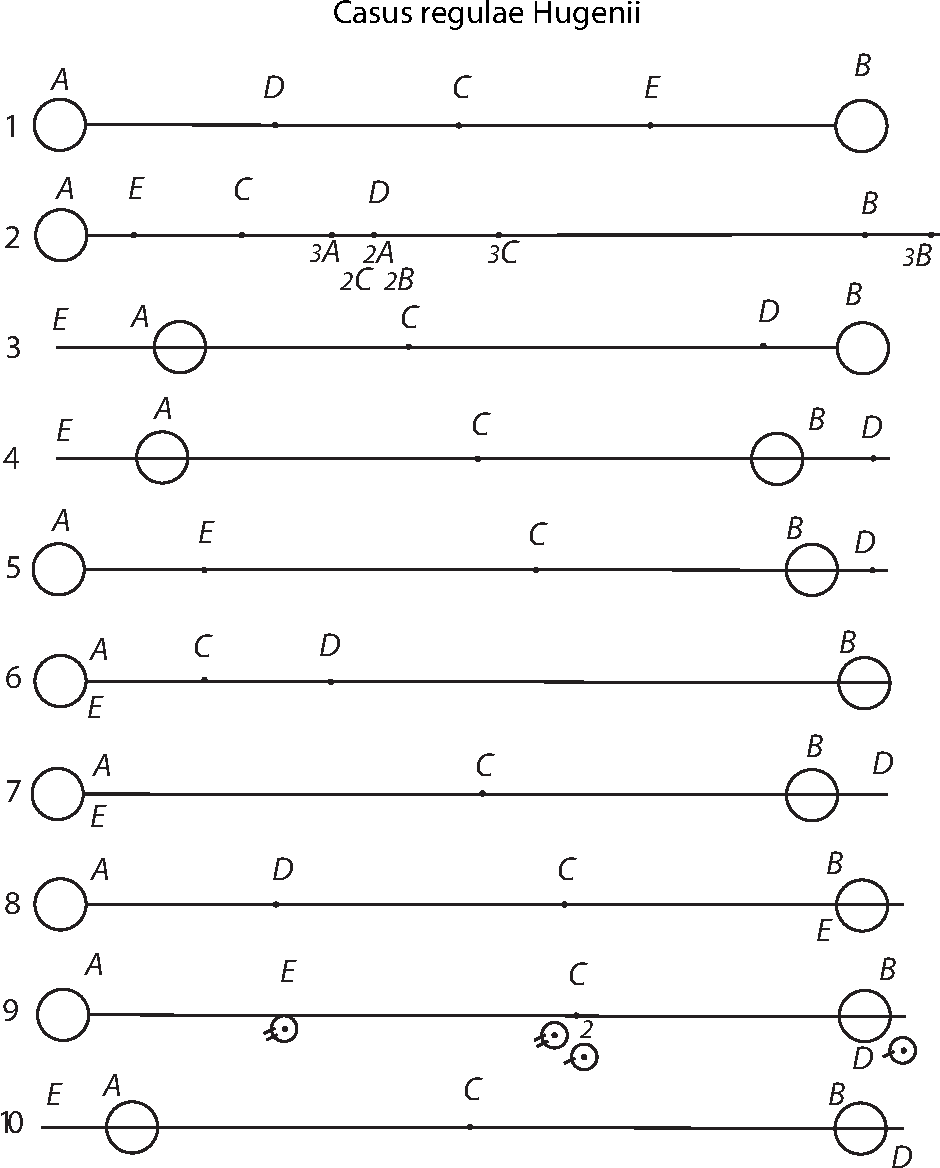
\includegraphics[width=0.75\textwidth]{%
gesamttex/edit_VIII,3/images/LH_37_05_144-145_d1_144v.pdf%
}} 
\vspace{0.5em}
%
\pstart
\centerline{%
\lbrack\textit{Fig.~1}\rbrack%
}
% \newpage%
\vspace{1.5em}
\edtext{}{% TRICK für ZEICHNUNG
\lemma{\hspace*{1,6mm}%
\lbrack\textit{Fig.~1}\rbrack%
}\killnumber%
\Cfootnote{%
Das Diagramm ist Huygens' Aufsatz entnommen (S.~23). Leibniz hat folgende Elemente ergänzt: die Nummern 1 bis 10 zur Bezeichnung der Fälle; im 2.\ Fall, die Verlängerung der Strecke rechts von \textit{B} sowie die Punkte \textit{{\scriptsize 2}A}, \textit{{\scriptsize 2}B}... \textit{{\scriptsize 3}C}; im 9.\ Fall, die Zahl \textit{2} und die Kreise unterhalb der Linie \textit{AB}.%
}}%
\pend
\newpage
\pstart
\hspace{1mm}\hspace{-1mm}% Trick, weil \edlabel nicht zu \par-Beginn sein darf
\edlabel{37_05_144-145_5a}\edtext{}{% C-Footnote – Huygens-Stelle
{\xxref%
{37_05_144-145_5a}{37_05_144-145_5b}}%
\lemma{\textit{Mais} \lbrack...\rbrack\ \textit{mouvemens}}%
\Cfootnote{%
\cite{00529}a.a.O., §2, S.~22.%
}}%
\textit{Mais si cet autre corps égal est aussi en mouvement, et qu'il soit porté dans la même ligne droite}\lbrack,\rbrack\ 
%
\textit{ils font un echange reciproque de} 
%
\edtext{\textit{leur}\lbrack\textit{s}\rbrack}{\lemma{}\Bfootnote{leur \textit{L ändert}\ \textit{Hrsg.}\ \textit{nach Vorlage}}}
%
\textit{mouvemens.\protect\index{Sachverzeichnis}{echange reciproque de mouvemens}}\edlabel{37_05_144-145_5b}
\pend %
%
\pstart
\hspace{1mm}\hspace{-1mm}% Trick, weil \edlabel nicht zu \par-Beginn sein darf
\edlabel{37_05_144-145_6a}\edtext{}{% C-Footnote – Huygens-Stelle
{\xxref%
{37_05_144-145_6a}{37_05_144-145_6b}}%
\lemma{\textit{Un corps} \lbrack...\rbrack\ \textit{mouvement}}%
\Cfootnote{%
\cite{00529}a.a.O., §3, S.~22.%
}}%
\textit{Un corps quelque petit
qu'il soit et quelque peu de vitesse qu'il ait, en rencontrant un autre plus grand qui soit en repos luy donnera quelque mouvement.}\edlabel{37_05_144-145_6b} 
\pend %
\pstart
%
\hspace{1mm}\hspace{-1mm}% Trick, weil \edlabel nicht zu \par-Beginn sein darf
\edlabel{37_05_144-145_7a}\edtext{}{% C-Footnote – Huygens-Stelle
{\xxref%
{37_05_144-145_7a}{37_05_144-145_7b}}%
\lemma{\textit{La quantité} \lbrack...\rbrack\ \textit{contraire}}%
\Cfootnote{%
\cite{00529}a.a.O., §5, S.~23.%
}}%
\textit{La} \edtext{\textit{quantité du mouvement}\protect\index{Sachverzeichnis}{quantité du mouvement}}{\lemma{\textit{quantité}}\Bfootnote{\textit{(1)}~de mou \textit{(2)}~\textit{du mouvement}~\textit{L}}}
%
\textit{qu'ont deux corps se peut augmenter et diminuer par leur rencontre,%
\protect\index{Sachverzeichnis}{rencontre}}  
%
\textit{mais il y reste tousjours la même quantité vers le même costé, en soustrayant la quantité}  
%
\textit{du mouvement\protect\index{Sachverzeichnis}{quantité du mouvement} contraire.}\edlabel{37_05_144-145_7b}
\pend %
\pstart
\hspace{1mm}\hspace{-1mm}% Trick, weil \edlabel nicht zu \par-Beginn sein darf
\edlabel{37_05_144-145_8a}\edtext{}{% C-Footnote – Huygens-Stelle
{\xxref%
{37_05_144-145_8a}{37_05_144-145_8b}}%
\lemma{\textit{La somme} \lbrack...\rbrack\  \textit{rencontre}}%
\Cfootnote{%
\cite{00529}a.a.O., §6, S.~23.%
}}%
\textit{La somme des produits faits de la grandeur de chaque corps dur%
\protect\index{Sachverzeichnis}{corps dur}}  
%
\textit{multiplié par le quarré de sa vitesse,\protect\index{Sachverzeichnis}{quarré de la vitesse}\protect\index{Sachverzeichnis}{produit de la grandeur par le quarré de la vitesse} est tousjours la même devant}  
%
\textit{et après leur rencontre.\protect\index{Sachverzeichnis}{rencontre}}\edlabel{37_05_144-145_8b}
\pend %
\pstart
\hspace{1mm}\hspace{-1mm}% Trick, weil \edlabel nicht zu \par-Beginn sein darf
\edlabel{37_05_144-145_9a}\edtext{}{% C-Footnote – Huygens-Stelle
{\xxref%
{37_05_144-145_9a}{37_05_144-145_9b}}%
\lemma{\textit{Un corps} \lbrack...\rbrack\ \textit{repos}}%
\Cfootnote{%
\cite{00529}a.a.O., §7, S.~23.%
}}%
\textit{Un corps dur qui est en repos receuvra plus de mouvement par un autre corps dur plus grand ou moindre que luy par} 
%
\edtext{\lbrack\textit{l'}\rbrack}{%
\lemma{un}%
\Bfootnote{\textit{L ändert Hrsg.\ nach Vorlage}%
}}%
\textit{interposition\protect\index{Sachverzeichnis}{corps interposé} d'un tiers de grandeur moyenne, que s'il en etoit frappé immediatement, et si}  
%
\edtext{\lbrack\textit{ce}\rbrack}{%
\lemma{}%
\Bfootnote{%
\textit{ce} %
\textit{erg.\ Hrsg.\ nach Vorlage}%
}}
\textit{corps interposé\protect\index{Sachverzeichnis}{corps interposé} est %
moyen proportionel\protect\index{Sachverzeichnis}{moyen proportionel} entre les deux 
autres il fera le plus d'impression sur celuy qui est en repos.}\edlabel{37_05_144-145_9b}
\pend \pstart
\hspace{1mm}\hspace{-1mm}% Trick, weil \edlabel nicht zu \par-Beginn sein darf
\edlabel{37_05_144-145_10a}\edtext{}{% C-Footnote – Huygens-Stelle
{\xxref%
{37_05_144-145_10a}{37_05_144-145_10b}}%
\lemma{\textit{Je} \lbrack...\rbrack\ \textit{autres}}%
\Cfootnote{%
\cite{00529}a.a.O., S.~23.%
}}%
\textit{Je considere en tout cecy des corps d'une même matiere, ou bien j'entends que leur grandeur
soit estimée par le poids%
\protect\index{Sachverzeichnis}{poids}.}
\pend  
%
\pstart
\textit{Au reste j'ay remarqué une loix admirable de la nature\protect\index{Sachverzeichnis}{loix admirable de la nature},
la quelle je puis demonstrer en ce qui est des corps spheriques,%
\protect\index{Sachverzeichnis}{corps sphérique} et qui semble estre
generale en tous les autres,}\edlabel{37_05_144-145_10b}
%
\edlabel{37_05_144-145_11a}\edtext{}{% C-Footnote – Huygens-Stelle
{\xxref%
{37_05_144-145_11a}{37_05_144-145_11b}}%
\lemma{\textit{ta}}%
\Cfootnote{%
\hspace{-2.4mm}\textit{nt} \lbrack...\rbrack\  \textit{rencontre}: \hspace{1mm}\cite{00529}a.a.O., S.~24.%
}}%
\textit{tant durs%
\protect\index{Sachverzeichnis}{corps dur} que mols,%
\protect\index{Sachverzeichnis}{corps mou} soit que la rencontre soit directe%
\protect\index{Sachverzeichnis}{rencontre directe} ou oblique:%
\protect\index{Sachverzeichnis}{rencontre oblique} c'est que le} 
%
\edtext{\textit{centre commun}}{\lemma{\textit{centre}}\Bfootnote{\textit{(1)}~de gravité \textit{(2)}~\textit{commun}~\textit{L}}}
%
\textit{de gravité\protect\index{Sachverzeichnis}{centre commun de gravité} de deux ou de trois, ou de tant qu'on voudra de corps avance tousjours}
%
\edtext{\textit{également vers}}{\lemma{\protect{\textit{également}}}\Bfootnote{\textit{(1)}~en même \textit{(2)}~\textit{vers}~\textit{L}}}
%
\textit{le même costé en ligne}  
%
\edtext{\lbrack\textit{droite}\rbrack,}{%
\lemma{}%
\Bfootnote{%
directe %
\textit{L ändert Hrsg.\ nach Vorlage}%
}}
%
\textit{devant et après leur rencontre.\protect\index{Sachverzeichnis}{rencontre}}\edlabel{37_05_144-145_11b}
\pend 
%
\selectlanguage{latin}
\frenchspacing
\pstart
\edtext{Haec habet Hugenius\protect\index{Namensregister}{\textso{Huygens} (Hugenius, Ugenius, Hugens, Huguens), Christiaan 1629\textendash1695}
%
in \textit{Diario Eruditorum} 9 Decembris 1669.}{\lemma{Haec \lbrack...\rbrack\ 1669}\Cfootnote{Es gab keine Lieferung des \cite{00157}\textit{JS} am 9.~Dezember 1669. Huygens' Aufsatz\cite{00529} erschien in der Ausgabe vom 18.~März und dessen lateinische Übersetzung\cite{01067} in den \cite{00158}\textit{PT} vom 12.~(22.)~April 1669.%
}}
%
\pend %
\pstart
Cum vero mihi semper visum sit, et etiamnum videatur potentiam,%
\protect\index{Sachverzeichnis}{potentia} seu motus absoluti quantitatem\protect\index{Sachverzeichnis}{quantitas motus absoluti} neque augeri neque minui posse, quia si augeretur, statim inde motus perpetuus Mechanicus\protect\index{Sachverzeichnis}{motus perpetuus Mechanicus} consequeretur, ideo
Decem casus Hugenianos\protect\index{Namensregister}{\textso{Huygens} (Hugenius, Ugenius, Hugens, Huguens), Christiaan 1629\textendash1695}%
\protect\index{Sachverzeichnis}{decem casus Hugeniani} ad hoc principium meum\protect\index{Sachverzeichnis}{principium meum} exigam.
\pend 
\newpage
\pstart
\hspace{1mm}\hspace{-1mm}% Trick, weil \edlabel nicht zu \par-Beginn sein darf
\edlabel{37_05_144-145_25a}%	zwecks Referenzierung
Si ponamus eandem quantitatem motus\protect\index{Sachverzeichnis}{quantitas motus} 
servari ante et post %
concursum\protect\index{Sachverzeichnis}{concursus},
erit \textit{AE} in $BC,+BE$ in \textit{AC}
%
\edtext{aequ.\ \textit{AD}}{%
\lemma{}%
\Bfootnote{%
aequ.\ \textbar\ aequ.\ \textit{streicht Hrsg.}\ \textbar\ %
\textit{AD}~\textit{L}}}
%
in $BC+BD$ in \textit{AC}.%
\edlabel{37_05_144-145_25b} %	zwecks Referenzierung
%
Nam \textit{AC} 
%
\edtext{et \textit{BC} lineae representant}{\lemma{}\Bfootnote{et \textit{BC} \textbar\ lineae \textit{erg.}\ \textbar\ \textit{(1)}~representat \textit{(2)}~representant~\textit{L}}}
%
quantitatem corporum,%
\protect\index{Sachverzeichnis}{quantitas corporis} illud corporis \textit{B} hoc corporis \textit{A}, sunt enim
brachia%
\protect\index{Sachverzeichnis}{brachium} seu distantiae a centro gravitatis\protect\index{Sachverzeichnis}{centrum gravitatis} ut corpora
%
\edtext{reciproce. Ergo \textit{AD} celeritas corporis \textit{A} in}{\lemma{reciproce.}\Bfootnote{\textit{(1)}~Sunt autem \textit{AE} \textit{(2)}~Ergo \textit{AD} \textbar\ celeritas corporis \textit{A} \textit{erg.}\ \textbar\ in~\textit{L}}}
% 
\textit{BC} seu in corpus \textit{A} est
potentia\protect\index{Sachverzeichnis}{potentia} corporis \textit{A}, ante concursum;\protect\index{Sachverzeichnis}{concursus} et \textit{BD} celeritas corporis \textit{B}, in \textit{AC} seu in corpus \textit{B}, est potentia\protect\index{Sachverzeichnis}{potentia} 
corporis \textit{B} ante concursum\protect\index{Sachverzeichnis}{concursus}. Ergo \textit{AD} in $BC, + BD$ in \textit{AC} est potentia\protect\index{Sachverzeichnis}{potentia} utriusque corporis ante concursum.\protect\index{Sachverzeichnis}{concursus} Et quia post 
concursum\protect\index{Sachverzeichnis}{concursus} pro celeritatibus \textit{AD}, \textit{BD} substituuntur \textit{AE}, \textit{BE}, hinc \textit{AE} in $BC, + BE$ in \textit{AC}, sunt 
%
\edtext{\lbrack potentiae\rbrack\protect\index{Sachverzeichnis}{potentia}}{%
\lemma{potentia}%
\Bfootnote{\textit{L ändert Hrsg.}\ %
}}
%
utriusque corporis post concursum,\protect\index{Sachverzeichnis}{concursus} quas potentias\protect\index{Sachverzeichnis}{potentia} suppono esse debere aequales.
\pend \pstart
\hspace{1mm}\hspace{-1mm}% Trick, weil \edlabel nicht zu \par-Beginn sein darf
\edlabel{37_05_144-145_26a}%	zwecks Referenzierung
Quia $AE \smallfrown BC, + BE \smallfrown AC \sqcap  AD \smallfrown BC + BD \smallfrown AC$. Ergo $ \underset{\displaystyle -AE}{+AD}, \smallfrown BC \sqcap \underset{\displaystyle -BD}{+BE} \smallfrown AC$. Seu $\displaystyle\frac{AC}{BC} \sqcap \displaystyle\frac{AD-AE}{BE-BD} \sqcap \displaystyle\frac{\textup{cor.}\ B}{\textup{cor.}\ A}$.%
\edlabel{37_05_144-145_26b} %	zwecks Referenzierung
%
Unde ex hypothesi nostra manentis potentiae,\protect\index{Sachverzeichnis}{hypothesis manentis potentiae} sequitur theorema\protect\index{Sachverzeichnis}{theorema pulchrum} mutationes 
\rule[0cm]{0mm}{10pt}%
celeritatum\protect\index{Sachverzeichnis}{mutatio celeritatis} per concursum\protect\index{Sachverzeichnis}{concursus}
%
\edtext{esse reciproce}{\lemma{esse}\Bfootnote{\textit{(1)}~\textbar\ ut \textit{streicht}\ \textit{Hrsg.}\ \textbar\ corpora \textit{(2)}~reciproce~\textit{L}}}
%
ut corpora concurrentia, quod et rationi%
\protect\index{Sachverzeichnis}{ratio} egregie consentaneum est, nam resistunt mutationi celeritatis%
\protect\index{Sachverzeichnis}{mutatio celeritatis} proportione magnitudinis. Nam cum magnitudo mutari non  
%
\edtext{possit, nihil}{\lemma{possit,}\Bfootnote{\textit{(1)}~necesse est ut \textit{(2)}~nihil~\textit{L}}}
%
aliud contribuere potest, quam ad conservationem celeritatis\protect\index{Sachverzeichnis}{conservatio celeritatis}, qua  
%
\edtext{sola ratione celeritates ergo perditae}{\lemma{sola ratione}\Bfootnote{\textit{(1)}~celeritas \textit{(2)}~celeritates ergo \textit{(a)}~conservatae \textit{(b)}~perditae~\textit{L}}}
%
sunt inter se in ratione  
%
\edtext{composita directa\protect\index{Sachverzeichnis}{ratio composita directa}}{%
\lemma{composita}%
\Bfootnote{%
\textit{(1)}~ex %
\textit{(2)}~directa %
\textit{L}%
}}
 ipsarum celeritatum, reciproca%
\protect\index{Sachverzeichnis}{ratio composita reciproca} magnitudinum. Hanc ergo aequationem
%
$\displaystyle\frac{AC}{BC} \sqcap \displaystyle\frac{DA-AE}{-DB+BE}$
%
\rule[0cm]{0mm}{16pt}%
decem Hugenii\protect\index{Namensregister}{\textso{Huygens} (Hugenius, Ugenius, Hugens, Huguens), Christiaan 1629\textendash1695} casibus\protect\index{Sachverzeichnis}{decem casus Hugeniani} applicemus:
\pend
\rule[0cm]{40mm}{0cm}%
\pstart
\hspace{1mm}\hspace{-1mm}% Trick, weil \edlabel nicht zu \par-Beginn sein darf
\edlabel{37_05_144-145_27a}%	und zwecks Referenzierung
\edtext{}{% C-Footnote – Fehler Vektoraddition
{\xxref%
{37_05_144-145_27a}{37_05_144-145_27b}}%
\lemma{1\textsuperscript{mo} \lbrack...\rbrack\ potest}%
\Cfootnote{%
Leibnizens Bewertung von Huygens' Ergebnissen als falsch oder ungewiss geht auf seine fehlerhafte Handhabung der Vorzeichen in der Vektoraddition zurück.%
}}%
1\textsuperscript{mo} casu $\displaystyle\frac{AC}{BC} \sqcap \displaystyle\frac{-DE}{-DE} \sqcap 1.$ Falsum
nam \textit{AB}, \textit{BC} inaequal.
\pend 
\rule[0cm]{40mm}{0cm}
\pstart
2\textsuperscript{do} casu 
%
$\displaystyle\frac{\edtext{\lbrack AC\rbrack}{%
\lemma{}%
\Bfootnote{%
\textit{AB} %
\textit{L ändert Hrsg.}\ %
}}
}{BC} \sqcap \displaystyle\frac{D E}{-DE}$ 
%
absurdum. Neque enim %
quantitas negativa\protect\index{Sachverzeichnis}{quantitas negativa} aequalis positivae.\protect\index{Sachverzeichnis}{quantitas positiva}
\pend
\rule[0cm]{40mm}{0cm}
 \pstart
3\textsuperscript{tio} casu 
%
$\displaystyle\frac{AC}{BC} \sqcap \displaystyle\frac{DA -AE}{DE}$ 
%
quod est dubium, id est non potest esse semper verum, ut hic \rule[0cm]{0mm}{12pt}%
dicitur.
\pend 
\newpage
\pstart
Quarto casu: 
%
\edtext{$\displaystyle\frac{AC}{BC} \sqcap \displaystyle\frac{DA-AE}{EB-BD}$ dub}{\lemma{$\displaystyle\frac{DA-AE}{EB-BD}$}\Bfootnote{\textit{(1)}~\Denarius\ \textit{(2)}~dub.~\textit{L}}}.
\pend
\rule[0cm]{40mm}{0cm}
 \pstart
5\textsuperscript{to} casu
%
\edtext{$\displaystyle\frac{AC}{BC} \sqcap \displaystyle\frac{D E}{EB-BD}$ 
dub}{\lemma{$\displaystyle\frac{D E}{EB-BD}$}\Bfootnote{\textit{(1)}~\Denarius\ \textit{(2)}~dub.~\textit{L}}}.
\pend 
\rule[0cm]{40mm}{0cm}
\pstart
6\textsuperscript{to} casu 
%
$\displaystyle\frac{AC}{BC} \sqcap \displaystyle\frac{DA}{ED \sqcap D A}$ 
%
falsum deberent enim \edtext{\lbrack\textit{AC}\rbrack,}{%
\lemma{}%
\Bfootnote{%
\textit{AB} %
\textit{L ändert Hrsg.}\ %
}}
 et \textit{BC} esse aequales. 
\pend 
\rule[0cm]{40mm}{0cm}
\pstart
7\textsuperscript{mo} casu 
%
$\displaystyle\frac{AC}{BC} \,\sqcap$
%
\edtext{\,$\displaystyle\frac{D A}{EB-BD}$ falsum, nam quia}{\lemma{ $\displaystyle\frac{D A}{EB-BD}$ }\Bfootnote{\textit{(1)}~falsum \textit{(2)}~dub. \textit{(3)}~falsum, \textit{(a)}~nam \textit{AB} \textit{(b)}~nam quia~\textit{L}}}
%
%
in hoc casu \textit{AC} aequ.\ \textit{CD} erit \textit{AC} plus quam 
\rule[0cm]{0mm}{12pt}%
duplum ipsius \edtext{\lbrack\textit{BC}\rbrack.}{%
\lemma{}%
\Bfootnote{%
\textit{CD}
\textit{L ändert Hrsg.}%
}}
 Sed \textit{DA} minor est duplo ipsius 
$EB - BD$. 
\pend 
\vspace{2mm}
\pstart
8\textsuperscript{vo} casu
%
$\displaystyle\frac{AC}{BC} \sqcap \displaystyle\frac{-D E}{-BD \sqcap -D E}$ 
%
falsum, quia \textit{AC} ac \textit{BC} non sunt aequales. 
\pend
\rule[0cm]{40mm}{0cm}
 \pstart
Nono casu
%
$\displaystyle\frac{AC}{BC} \sqcap \displaystyle\frac{DE}{EB \sqcap D E}$ 
%
falsum ob eandem rationem.
\pend
\rule[0cm]{40mm}{0cm}
 \pstart
10\textsuperscript{mo} casu
%
$\displaystyle\frac{AC}{BC} \sqcap \displaystyle\frac{DA - AE}{EB}$ 
%
falsum 
\edtext{plerumque}{%
\lemma{}%
\Bfootnote{%
plerumque %
\textit{erg.\ L}%
}}
%
nam $\displaystyle\frac{AC}{BC} \sqcap \displaystyle\frac{BC+CA-AE}{EA+AC+BC}$. 
%
Ergo 
%
$AC \smallfrown BA,, + AC \smallfrown AC,$ \rule[0cm]{0mm}{12pt}%
\ovalbox{$+AC \smallfrown BC$} $\sqcap\, BC \smallfrown BC,$ \ovalbox{$+BC\smallfrown AC$} $-BC \smallfrown AE$.
%
Ergo 
%
$AE \smallfrown AB \sqcap BC^2 - AC^2$, 
%
\rule[-2mm]{0mm}{8mm}sive erit
$AE \smallfrown AB \sqcap \underbrace{BC+AC}_{\displaystyle BA} \smallfrown BC - AC$.
%
Ergo
%
$BC - AC \sqcap AE$
%
quod tamen 
\rule[0cm]{0mm}{10pt}%
universaliter verum esse non potest.%
\edlabel{37_05_144-145_27b}%	zwecks Referenzierung
%
\pend
\vspace{0.5mm}
\pstart
\hspace{1mm}\hspace{-1mm}% Trick, weil \edlabel nicht zu \par-Beginn sein darf
%
\edlabel{37_05_144-145_19a}%
\edtext{}{% C-Footnote Kommentar Komma = Produkt
{\xxref%
{37_05_144-145_19a}{37_05_144-145_19b}}%
\lemma{Casu 7.\  \lbrack...\rbrack\  $\displaystyle\frac{BC+CD}{AC - BD}$}% LEMMA ANPASSEN
\Cfootnote{%
Leibniz verwendet hier das Komma als Multiplikationszeichen, neben dem üblicheren Zeichen $\smallfrown$\,.%
}}% KEIN LEERZEICHEN
\lbrack144~r\textsuperscript{o}\rbrack\ 
\textlangle\textendash\textrangle\ Casu 7.\
%
$\underbrace{BA}_{\displaystyle BC+CA}$ in \textit{AC}
%
seu
%
$BC,AC,,+AC^2,,$
%
debet esse $\underbrace{AD}_{\displaystyle AC+CB+BD}$ in $BC + BD$ in \textit{AC} \rule[-4mm]{0mm}{8mm}seu debet esse 
%
$AC,BC+BC^2+BD,%
\edtext{\lbrack BC\rbrack}{%
\lemma{\textit{AC}}%
\Bfootnote{%
\textit{L ändert Hrsg.}\ %
}}%
+BD,AC$.%
\pend
\vspace{-0.8mm}
\pstart
%
Ergo 
%
$\ovalbox{\textit{BC},\,\textit{AC}}, + AC^2\; \sqcap\; 
\rule[0cm]{0mm}{12pt}%
\ovalbox{\textit{AC},\,\textit{BC}},, + BC^2, + BD,BC,+ BD,AC$. 
%
\edtext{Seu $AC \smallfrown \underset{\displaystyle -BD}{+AC} \sqcap BC, \smallfrown BC + CD$.}{%
\lemma{Seu \lbrack...\rbrack\ $BC + CD$}%
\Cfootnote{%
Die rechte Seite der Gleichung heißt eigentlich $BC, \smallfrown BC + BD$. Der Fehler wirkt sich auf die folgende Umformung aus.}}
%
Ergo 
%
$\displaystyle\frac{AC}{BC} \sqcap \displaystyle\frac{BC+CD}{AC - BD}$.
\edlabel{37_05_144-145_19b}
\pend
%
%%%%%%%%%%%%%%%%%%%%%%%%%%%%%%%%%%%%%%%%%%%%%%
% Ende der Einfügung oberhalb. Textfolge überprüfen %%
%%%%%%%%%%%%%%%%%%%%%%%%%%%%%%%%%%%%%%%%%%%%%%
\newpage
\pstart
\lbrack145~r\textsuperscript{o}\rbrack\ 
%%%%%
% =1=
Hic ut obiter dicam notabile calculi exemplum%
\protect\index{Sachverzeichnis}{notabile exemplum calculi}
%
$\displaystyle\frac{x+y-z}{x+y+z}\ \sqcap\ \displaystyle\frac{y}{x}$.
%
Ergo 
%
$x^2\ovalbox{$+xy$}-zy \sqcap \ovalbox{$xy$}+y^2+zx$.
%
% =2=
%
Ergo
%
$\underbrace{x^2 - y^2}_{\displaystyle x+y \smallfrown x-y} \sqcap\ % 
%%%\edtext{\lbrack x+y\rbrack}{%	% 1. Möglichkeit: Hrsg-Eingriff
%%%\lemma{}%
%%%\Bfootnote{%
%%%$\protect\underset{\displaystyle +y}{+x}$ %
%%%\textit{L ändert Hrsg.}\ %
%%%}}
%
%%%\displaystyle\efrac{+x}{+y}	% 2. Möglichkeit: efrac (sieht aber nicht gut aus.)
\underset{\displaystyle +y}{+x} 		% 3. Möglichkeit: so lassen, wie es ist
\smallfrown z$.
%
Ergo
%
$x-y \sqcap z$.
%
\rule[0cm]{0mm}{12pt}%
Theorema ergo hoc est: si sit
%
$x + y - z$ ad $ x + y + z$ ut \textit{y} ad \textit{x}, 
%
tunc
%
% =3= %%%%%%%%
%
alterutrum necesse est, vel scilicet esse \textit{x} aequ.\ $-y$ vel 
%
$x \sqcap z+y$.
%
Ponendo autem literas
%%%%%%%%
%% =4= %%%
%%%%%%%%
omnes esse quantitates affirmativas%
\protect\index{Sachverzeichnis}{quantitas affirmativa} theorema erit: si sit $x+y-z$ ad $x+y+z$ ut \textit{y} ad \textit{x} erit \textit{x} aequ.\ $z+y$.
\pend 
%
\vspace{1.5em} %%%%%%%%% Diagramm  2
\centerline{%
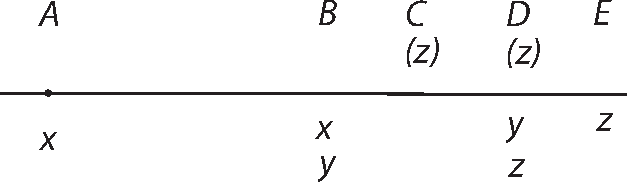
\includegraphics[width=0.5\textwidth]{%
gesamttex/edit_VIII,3/images/LH_37_05_144-145_d2_145r.pdf%
}} 
\vspace{0.5em}
\centerline{%
\lbrack\textit{Fig.~2}\rbrack%
}
% \newpage%
\vspace{1.5em}
%
%
\pstart
Sit 
%
\edtext{recta \textit{ABCDE} divisa ita ut}{%
\lemma{recta}\Bfootnote{\textit{(1)}~\textit{AE} \textit{(2)}~\textit{ABCDE} divisa \textit{(a)}~in \textit{(aa)}~quatuor \textit{(bb)}~tribus punctis \textit{B}, \textit{C}, \textit{D} \textit{(b)}~ita ut~\textit{L}}}  
%
sit \textit{CD} aequ.\ \textit{DE} et \textit{AC} ad totam \textit{A}\textlangle\textit{E}\textrangle\
%
% =6=
%
ut \textit{BD} ad \textit{AB}. Erit 
%
\textit{AB} aequ.\ \textit{BE}. Sed hoc obiter.
%
\pend \pstart
%
\edtext{Si Hugenii\protect\index{Namensregister}{\textso{Huygens} (Hugenius, Ugenius, Hugens, Huguens), Christiaan 1629\textendash1695} regula%
\protect\index{Sachverzeichnis}{regula Hugenii} esset vera,  
%
\edtext{quod facta}{%
\lemma{quod}%
\Bfootnote{%
\textit{(1)}~factum %
\textit{(2)}~facta%
~\textit{L}%
}}
ex corporibus in quadrata celeritatum,%
\protect\index{Sachverzeichnis}{factum ex corpore in quadratum celeritatis} simul addita, ante et post concursum%
\protect\index{Sachverzeichnis}{concursus}
%
% =8=
%
sint aequalia,}{%
\lemma{Si \lbrack...\rbrack\  aequalia}%
\Cfootnote{%
\cite{00529}a.a.O., §6, S.~23.}}
%
\rule[0cm]{0mm}{16pt}foret 
%
$\displaystyle\frac{AC}{BC} \sqcap \displaystyle\frac{DA^2-AE^2}{EB^2 - BD^2}$
%
tantum, enim pro ipsis celeritatibus calculi superioris substituenda
%
% == 9 ==
%
\rule[0cm]{0mm}{10pt}eorum quadrata.%
\protect\index{Sachverzeichnis}{quadratum celeritatis} (\protect\vphantom)+ Hoc exemplo ut obiter dicam intelligi potest, non esse saepe opus calculis, cum jam tum praedici 
%
% ==10==
%
potest quod sit proditurum ex simplici \rule[0cm]{0mm}{16pt}aequipollentia\lbrack+\protect\vphantom()\rbrack.%
\protect\index{Sachverzeichnis}{aequipollentia} Seu 
%
$\displaystyle\frac{AC}{BC} \sqcap \displaystyle\frac{DA+AE, \smallfrown DA - AE}{EB+BD, \smallfrown EB-BD}$.
%
Ergo semper esse 
%
\edtext{deberent corpora reciproce in}{\lemma{deberent}\Bfootnote{\textit{(1)}~summae \textit{(2)}~corpora \textit{(a)}~in reciproca \textit{(b)}~reciproce in~\textit{L}}}
%
% ==11==
%
%\rule[0cm]{0mm}{10pt}
composita ratione ex summis%
\protect\index{Sachverzeichnis}{summa celeritatum priorum et posteriorum} et differentiis celeritatum priorum et posteriorum.\protect\index{Sachverzeichnis}{differentia celeritatum priorum et posteriorum} Ponamus esse
%
% == 12 ==
%
$DA+AE \sqcap DE$
%
(ad discernendum illum casum quo \textit{E} est inter \textit{E} et \textit{A}, vel \textit{D} inter \textit{A} et \textit{E}). Et ponamus eodem modo esse 
%
$EB + BD \sqcap ED$
%
% == 13 ==
%
id est si simul posita sint \textit{A} inter \textit{D} et \textit{E}, et \textit{B} quoque inter \textit{D} et \textit{E}, erit $DA + AE$ aequ.\ $EB+BD$, erit\rule[0cm]{0mm}{16pt}
%
$\displaystyle\frac{AC}{BC} \sqcap \displaystyle\frac{DA - AE}{EB - BD}$,
%
et
%
% == 14 ==
%
hoc casu regula Hugeniana\protect\index{Sachverzeichnis}{regula Hugeniana}
coincidet
\pend
\newpage
\pstart
\noindent cum nostra.\protect\index{Sachverzeichnis}{regula nostra} 
%
\edlabel{37_05_144-145_29a}%	zwecks Referenzierung
Et hoc fit casu 4\textsuperscript{to}, 7\textsuperscript{mo} et 10\textsuperscript{mo}. 
\rule[0cm]{0mm}{10pt}Ergo secundum hanc 
%
\edtext{regulam Hugenii\protect\index{Namensregister}{\textso{Huygens} (Hugenius, Ugenius, Hugens, Huguens), Christiaan 1629\textendash1695}}{\lemma{regulam}\Bfootnote{\textit{(1)}~Hugenii decisio quam affert casu \textit{(2)}~Hugenii~\textit{L}}}
%
% == 15 ==
%
solutio casuum 4, 7, 10 debet coincidere cum nostra.%
\protect\index{Sachverzeichnis}{solutio nostra}%
\edlabel{37_05_144-145_29b} %	zwecks Referenzierung
%
Et tamen supra determinavimus regulas Hugenii\protect\index{Namensregister}{\textso{Huygens} (Hugenius, Ugenius, Hugens, Huguens), Christiaan 1629\textendash1695}%
 \protect\index{Sachverzeichnis}{regulae Hugenii} fallere secundum nostram Hypothesin in casu 7, 10. Ergo regulae Hugenii\protect\index{Namensregister}{\textso{Huygens} (Hugenius, Ugenius, Hugens, Huguens), Christiaan 1629\textendash1695} \protect\index{Sachverzeichnis}{regulae Hugenii} in hoc
% 
% == 17 ==
%
quidem casu ne sibi quidem ipsis constant. 
%
\edlabel{37_05_144-145_28a}%	zwecks Referenzierung
\edtext{Quod ipsi Hugenio\protect\index{Namensregister}{\textso{Huygens} (Hugenius, Ugenius, Hugens, Huguens), Christiaan 1629\textendash1695} significare operae pretium esse videtur.}{%
\lemma{Quod \lbrack...\rbrack\ videtur}%
\Cfootnote{%
Aus dem Zeitraum Juli 1676 bis Mitte September 1679 sind keine Briefe zwischen Leibniz und Huygens bekannt.}}%
\edlabel{37_05_144-145_24b}%Ende der Besprechung von Huygens
\edlabel{37_05_144-145_28b}%	zwecks Referenzierung
%
% == 18 ==
%
\pend 
\count\Bfootins=1200%
\count\Afootins=1200%
\count\Cfootins=1200
%